\documentclass[paper=letter,fontsize=11pt]{scrartcl} % KOMA-article class
\usepackage[english]{babel}
\usepackage[utf8x]{inputenc}
\usepackage[protrusion=true,expansion=true]{microtype}
\usepackage{amsmath,amsfonts,amsthm}     % Math packages
\usepackage{graphicx}                    % Enable pdflatex
\usepackage[svgnames]{xcolor}            % Colors by their 'svgnames'
\usepackage{geometry}
	%\textheight=700px                    % Saving trees ;-)
%\usepackage{url}
\usepackage[colorlinks=true,
linkcolor=blue,
urlcolor=blue]{hyperref}
\usepackage{float}
\usepackage{etaremune}
\usepackage{wrapfig}
\usepackage{framed,graphicx,xcolor}
\definecolor{shadecolor}{rgb}{0.85,0.85,1}

\usepackage{attachfile}

\frenchspacing              % Better looking spacings after periods
\pagestyle{empty}           % No pagenumbers/headers/footers

%\addtolength{\voffset}{-40pt}
%\addtolength{\textheight}{20pt}

\setlength\topmargin{0pt}
\addtolength\topmargin{-\headheight}
\addtolength\topmargin{-\headsep}
\setlength\oddsidemargin{0pt}
\setlength\textwidth{\paperwidth}
\addtolength\textwidth{-2in}
\setlength\textheight{\paperheight}
%\addtolength\textheight{-3in}
\addtolength\textheight{-2in}
\usepackage{layout}

%%% Custom sectioning}{sectsty package)
%%% ------------------------------------------------------------
\usepackage{sectsty}

\sectionfont{%			            % Change font of \section command
	\usefont{OT1}{phv}{b}{n}%		% bch-b-n: CharterBT-Bold font
	\sectionrule{0pt}{0pt}{-5pt}{3pt}}

%%% Macros
%%% ------------------------------------------------------------
\newlength{\spacebox}
\settowidth{\spacebox}{8888888888}			% Box to align text
\newcommand{\sepspace}{\vspace*{1em}}		% Vertical space macro

\newcommand{\MyName}[1]{ % Name
		\Huge \usefont{OT1}{phv}{b}{n} \hfill #1
		\par \normalsize \normalfont}

\newcommand{\MySlogan}[1]{ % Slogan}{optional)
		\large \usefont{OT1}{phv}{m}{n}\hfill \textit{#1}
		\par \normalsize \normalfont}

\newcommand{\NewPart}[2]{\section*{\uppercase{#1} #2}}

\newcommand{\PersonalEntry}[2]{
		\noindent\hangindent=2em\hangafter=0 % Indentation
		\parbox{\spacebox}{        % Box to align text
		\textit{#1}}		       % Entry name}{birth, address, etc.)
		\hspace{1.5em} #2 \par}    % Entry value

\newcommand{\SkillsEntry}[2]{      % Same as \PersonalEntry
		\noindent\hangindent=2em\hangafter=0 % Indentation
		\parbox{\spacebox}{        % Box to align text
		\textit{#1}}			   % Entry name}{birth, address, etc.)
		\hspace{1.5em} #2 \par}    % Entry value

\newcommand{\EducationEntry}[4]{
		\noindent \textbf{#1} \hfill      % Study
		\colorbox{White}{%
			\parbox{10em}{%
			\hfill\color{Black}#2}} \par  % Duration
		\noindent \textit{#3} \par        % School
		\noindent\hangindent=2em\hangafter=0 \small #4 % Description
		\normalsize \par}

\newcommand{\WorkEntry}[4]{				  % Same as \EducationEntry
		\noindent \textbf{#1} \hfill      % Jobname
		\colorbox{White}{\color{White}#2} \par  % Duration
		\noindent \textit{#3} \par              % Company
		\noindent\hangindent=2em\hangafter=0 \small #4 % Description
		\normalsize \par}

\newcommand{\PaperEntry}[7]{
		\noindent #1, ``\href{#7}{#2}", \textit{#3} \textbf{#4}, #5 (#6).}


\newcommand{\ArxivEntry}[3]{
		\noindent #1, ``\href{http://arxiv.org/abs/#3}{#2}", \textit{{cond-mat/}#3}.}

\newcommand{\BookEntry}[4]{
		\noindent #1, ``\href{#3}{#4}", \textit{#3}.}

\newcommand{\FundingEntry}[5]{
        \noindent #1, ``#2", \$#3 (#4, #5).}

\newcommand{\TalkEntry}[4]{
		\noindent #1, #2, #3 #4}

\newcommand{\ThesisEntry}[5]{
		\noindent #1 -- #2 #3 ``#4" \textit{#5}}

\newcommand{\CourseEntry}[3]{
		\noindent \item{#1: \textbf{#2} \\ #3}}

%%% Begin Document
%%% ------------------------------------------------------------
\begin{document}

%\layout

% you can upload a photo and include it here...
\begin{wrapfigure}{l}{0.5\textwidth}
	\vspace*{-2em}
		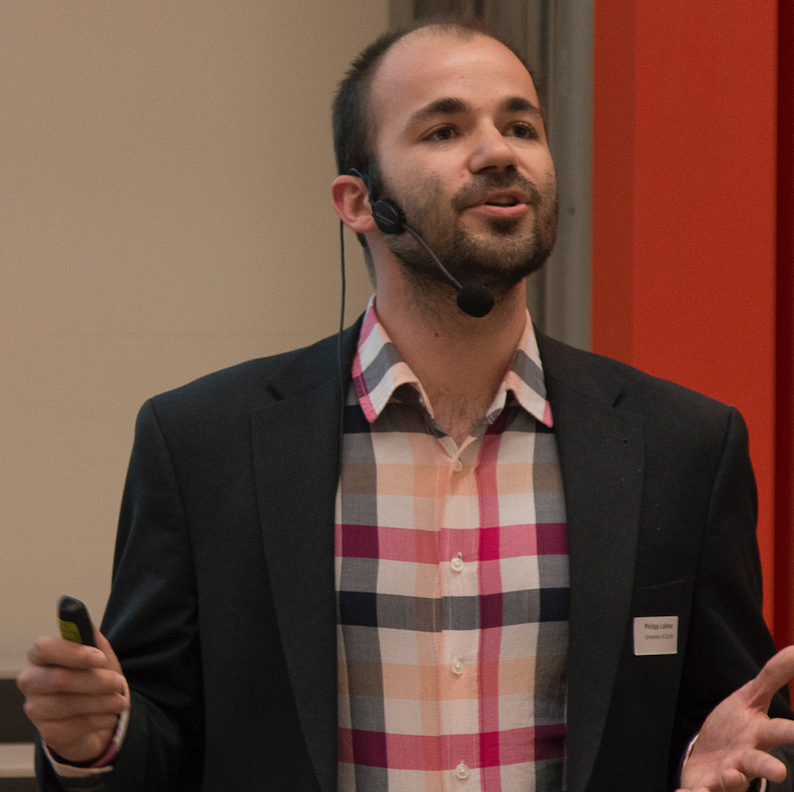
\includegraphics[width=0.18\textwidth]{profile.png}
\end{wrapfigure}

\MyName{Philipp Leitner}
\MySlogan{Academic Activities (\today)}

\sepspace

\NewPart{Acquired Grants}{}

\begin{itemize}
        \item Debloating AI Systems (2021), AoA SEED Grant\\
        Co-applicant\\
        Total budget 296,000 SEK (my part $\approx$128,000 SEK)\\
        ($\approx$ 13.000 EUR)
	\item FFI TrafCloud (2019 -- 2021), VINNOVA\\
	Co-applicant\\
	Chalmers budget 5,500,000 SEK (my part $\approx$3,200,000 SEK)\\
  ($\approx$ 315.000 EUR)
  \item VR Starting Grant (2019 -- 2022), VR\\
  Sole applicant\\
	Grant value 3,639,000 SEK\\
  ($\approx$ 359.000 EUR)
  \item WASP Academic PhD Student (2017 -- 2021), WASP\\
  Academic Supervisor\\
	Grant value $\approx$3,600,000 SEK\\
  ($\approx$ 355.000 EUR)
  \item Chalmers AoA Hiring Startup Package (2017 -- 2021), Chalmers Foundation\\
	Sole recepient\\
  Grant value 8,000,000 SEK\\
  ($\approx$ 789.000 EUR)
  \item Individual Project ``MINCA'' (2016 -- 2019), Swiss National Science Foundation\\
  Sole applicant \\
  Grant value 180,000 CHF, at University of Zurich\\
  ($\approx$ 163.000 EUR)
  \item Technology Transfer Project ``DevCloud'' (2016 -- 2019), Hasler Foundation\\
  Co-applicant \\
  Grant value 50,000 CHF, at University of Zurich\\
  ($\approx$ 45.000 EUR)
\end{itemize}

\NewPart{Research Visits}{}

  \begin{tabular}{p{12cm}l}
    Institute of of High-Performance Computing, Singapore & Feb./Mar. 2013 \\
    University of Stuttgart, Germany & Apr. 2010 \\
  \end{tabular}

% \NewPart{Past Faculty Applications}{}
%
% As requested by the SNF, I list all past faculty applications for which I
% have been invited to interviews or have been short-listed.
%
% \begin{itemize}
% \item Tenure-Track Assistant Professor at \textbf{University of Copenhagen},
% interview declined for personal reasons.
% \item Tenure-Track Assistant Professor at \textbf{Vrije Universiteit Amsterdam},
% interviewed Nov. 23rd, 2015. Ranked 2nd of 48 candidates.
% \item Tenure-Track Assistant Professor at \textbf{University of Gothenburg /
% Chalmers}, interviewed Jun. 16th, 2015. On 5-person short list of 25 candidates.
% \item Tenure-Track Research Assistant Professor at \textbf{IMDEA Madrid},
% interviewed Apr. 9th, 2013.
% \end{itemize}

\NewPart{Invited Talks and Seminars}{}

\begin{itemize}
  \item \emph{Unit testing performance using code microbenchmarks. How far are we?}, Invited Talk at the MongoDB Inc. Performance Seminar, November 2020
	\item \emph{Performance stability of (public) clouds}, Invited Talk at Vehicle Electronics and Connected Services (VECS, industrial conference), April 2019
	\item \emph{AWS Lambda and \#serverless. What’s all the fuzz about?}, Invited Talk at the Chaos Engineering Days Stockholm, December 2018
		\item \emph{Software performance testing in a public cloud – how bad is it really?}, Invited Talk at the Metrics Day 2018, October 2018
		\item \emph{Performance Testing of and in the Cloud}, Invited Lecture at the IDEA League Doctoral School on Engineering Complex Systems and IT with Big data and Information Technology, September 2018
\item \emph{Predictability of Performance in Public Clouds - Some Empirical Data and Lessons Learned for Software Performance Testing}, Seminar at IBM Research, Ireland, November 2017
\item \emph{Predictability of Performance in Public Clouds - Some Empirical Data and Lessons Learned for Software Performance Testing}, Invited Talk at the Sixth International Workshop on Load Testing and Benchmarking of Software Systems (LTB 2017), co-located with ICPE'17, April 2017
\item \emph{Your User is the Canary - Practices of and Obstacles to Conducting Experiments in Production}, CHOOSE Forum, University of Zurich, September 2016
\item \emph{How Predictable is the Performance of IaaS Instances? Some Insights from Benchmarking EC2, GCE, Azure, and Softlayer}, Open Cloud Day, ZHAW Winterthur, June 2016
\item \emph{Software Development for the Cloud – Challenges and Opportunities}, Faculty of Informatics, University of Lugano, February 2016
\item \emph{Software Development for the Cloud – Challenges and Opportunities}, VU University Amsterdam, November 2015
\item \emph{Trends, Opportunities and Challenges of Software Development for the Cloud}, Indian Institute of Technology Ropar, November 2015
\item \emph{Trends, Opportunities and Challenges of Software Development for the Cloud}, Indian Institute of Technology New Delhi, November 2015
\item \emph{Software Development for the Cloud -- Challenges and Opportunities}, Chalmers, Gothenburg, June 2015
\item \emph{Engineering Java Applications for the Infrastructure-as-a-Service Cloud}, software evolution \& architecture lab, University of Zurich, Zurich, October 2013
\item \emph{Building Applications for the Infrastructure-as-a-Service Cloud with CloudScale}, IMDEA Software Institute, Madrid, April 2013
\item \emph{Building Elastic Java Applications based on CloudScale and the Infrastructure-as-a-Service Paradigm}, National University of Singapore, School of Computing, March 2013
\item \emph{Building Elastic Java Applications based on CloudScale and the Infrastructure-as-a-Service Paradigm}, University of Illinois Advanced Digital Sciences Center, Singapore, February 2013
\end{itemize}

\NewPart{Awards}{}
\begin{itemize}
\item Distinguished Reviewer Award (ICSME 2020)  
\item Distinguished Reviewer Award (MSR 2020)
\item Outstanding Reviewer Award (ICPE 2020)
\item Outstanding Reviewer Award (ICPE 2019)
\item Best Student Paper Award (Middleware 2016)
\item Best Short Paper Award (ICPC 2016)
\end{itemize}


\NewPart{Department Service}{}
\begin{itemize}
\item Master Program Administrator Software Engineering (Chalmers and the University of Gothenburg, from 2021)
\item Member of the Faculty Senate Drafting Board (IT Faculty, University of Gothenburg, 2021 - 2024)
\item Postdoc Representative at the Department of Informatics, University of Zurich (2015 - 2016)
\item Member of the Habilitation Committee of Ivona Brandic (TU Vienna, 2013)
\item Member of the Habilitation Committee of Karl Michael G\"oschka (TU Vienna, 2012)
\end{itemize}

\NewPart{Professional Service}{}

\subsection*{Organized Events}
\begin{itemize}
\item Co-Organizer of the 1st and 2nd \emph{Vienna Software Seminar (VSS)} on the Relation of Software Architecture and DevOps/Continuous Delivery. Organizers: Uwe Zdun, Philipp Leitner, Florian Rosenberg, Erik Wittern.
\item Member of the Steering Committee of the International Workshop on Quality-Aware DevOps (QUDOS). From 2018.
\item Dagstuhl GI Seminar on \emph{Software Performance Engineering in the DevOps World} (September 26th – September 30th 2016, Schloss Dagstuhl, Germany). Co-organized with Andre van Hoorn, Pooyan Jamshidi, and Ingo Weber.
\item Half-day \emph{CloudWave Training Event} (September 5th 2016, TU Vienna, Austria). Half-day session at ESOCC'16. Co-organized with Andreas Metzger and Eliot Salant.
\end{itemize}

\subsection*{Editorial Memberships}
\begin{itemize}
\item Academic Editor of PeerJ Computer Science
\item Editorial Board Member of Elsevier's Journal on Systems and Software (JSS). Responsible for coordinating and implementing the publicity efforts of the journal. 2017 - 2019.
\item Special Issue Editor for "Converging Fog and Cloud Computing", in IEEE Cloud Computing. Co-edited with Erik Elmroth, Stefan Schulte, and Srikumar Venugopal.
\item Special Issue Editor for "Software Tools and Technologies for Monitoring and Prediction of Cloud Services", in Software: Practice and Experience (published by Wiley-Blackwell). Co-edited with Rajiv Ranjan, Raj\-kumar Buyya, Armin Haller, and Stefan Tai
\end{itemize}

\subsection*{Chairmanships}
\begin{itemize}
\item Program Co-Chair of 13th ACM/SPEC International Conference on Performance Engineering (ICPE) 
\item Awards Co-Chair of 12th ACM/SPEC International Conference on Performance Engineering (ICPE)
\item Publication Chair of 10th ACM/SPEC International Conference on Performance Engineering (ICPE)
\item PC Co-Chair of the  3rd International Workshop on Quality-Aware DevOps (QUDOS), co-located with the  8th ACM/SPEC International Conference on Performance Engineering (ICPE 2017)
\item Co-Chair of a Special Session on Services Computing and Internet Technologies (SerCo 2016) at the International Conference on High Performance Computing \& Simulation (HPCS 2016)
\item Tutorial Chair of the 16th International Conference on Web Engineering (ICWE2016)
\item Workshop Chair of the European Conference on Service-Oriented
and Cloud Computing (ESOCC) 2015.
\item General Chair of the 1st International Workshop on Monitoring and
Prediction of Cloud Services (MoPoC'12), co-located with ICSOC'12.
\end{itemize}


\subsection*{Reviews for Funding Agencies}

\begin{itemize}
	\item Dutch Research Council (NWO)
  \item Natural Sciences and Engineering Research Council of Canada (NSERC)
	\item Deutscher Akademischer Austauschdienst (DAAD)
	\item Luxembourg National Research Fund (FNR)
\end{itemize}

\subsection*{Program Commitee Memberships}

(partial list)

\begin{itemize}
	\item IEEE International Conference on Cloud Engineering (IC2E 2021)
	\item European Symposium on Serverless Computing and Applications (ESSCA 2020)
	\item International Conference on Microservices (MICROSERVICES 2020)
	\item IEEE/ACM International Conference on Automated Software Engineering - Demonstration Track (ASE 2019)
	\item IEEE International Conference on Software Analysis, Evolution and Reengineering (SANER, from 2019)
	\item IEEE International Conference on Software Maintenance and Evolution (ICSME, from 2018)
	\item International Conference on Mining Software Repositories (MSR, from 2018)
  \item ACM International Conference on Distributed Event-Based Systems (DEBS 2018)
	\item ACM/SPEC International Conference on Performance Engineering (ICPE 2018, 2020)
	\item IEEE International Conference on Cloud Computing (CLOUD, 2015 -- 2018)
	\item International Conference on the Quality of Information and Communications Technology (QUATIC, 2018)
	\item International Conference on Edge Computing (EDGE 2017)
  \item International Symposium on Fog and Edge Computing (ISFEC 2017)
	\item Euromicro Conference on Software Engineering and Advanced Applications (SEAA, 2018)
	\item International Conference on Service-Oriented Computing (ICSOC, 2015 -- 2017)
  \item European Conference on Service-Oriented and Cloud Computing (ESOCC, 2015, 2017)
  \item International Conference on Web Engineering (ICWE, 2015, 2019)
  \item IEEE/ACM International Utility and Cloud Computing Conference (UCC, 2014 -- 2017)
  \item International Conference on Service Oriented Computing and Applications (SOCA, 2014 -- ongoing)
	\item Cloud Challenge, held in conjunction with UCC (2014)
	\item International Workshop on RESTFul Designs (WS-REST, co-located with WWW, 2018)
	\item International Workshop on Software Engineering Aspects of Continuous Development and New Paradigms of Software Production and Deployment (DEVOPS, 2018)
  \item International Workshop on Autonomous Control for Performance and Reliability Trade-offs in Internet of Services (ACPROSS, 2017)
	\item International Workshop on Inter-Organizational Processes (IOPs, 2016)
    \item  International Workshop on Big Data Software Engineering (BIGDSE, 2015 -- ongoing)
  \item EAI International Conference on Cloud, Networking for IoT Systems (CN4IoT, 2015)
  \item International Conference on Internet and Web Applications and Services (ICIW, 2014 -- 2015)
  \item International Conference on the Future Internet of Things and Cloud (FiCloud, 2014)
    \item International Conference on Service Oriented Computing (ICSOC) Demonstration Track (2014 -- ongoing)
    \item International Workshop on Federative and Interoperable Cloud Infrastructures (FedICI, 2014)
    \item International Workshop on Engineering Cloud Applications \& Services (EnCASE, 2014)
  \item Central-European Workshop on Services and their Composition (ZEUS, 2012 -- ongoing)
  \item International Workshop on Evolutionary Business Processes EVL-BP), co-located with EDOC (2011 -- 2013)
  \item International Workshop on Principles of Engineering Service-Oriented Systems (PESOS), co-located with ICSE (2013)
  \item Track on Provisioning and Management of Service Oriented Architecture and Cloud Computing (PROMASC), a Track of the WETICE (2011 -- 2012)
  \item International Workshop on Performance Assessment and Auditing in Service Computing (PAASC), co-located with ICSOC (2011 -- 2012)
  \item Workshop on Emerging Web Services Technology (WEWST), co-located
  with ECOWS (2009 -- 2011)
  \item International Workshop on Dynamic and Declarative Business
  Processes (DDBP), co-located with EDOC (2010)
\end{itemize}

\subsection*{Reviews for Journals}

(partial list)

\begin{itemize}
\item Elsevier Information and Software Technology (IST)
\item IEEE Transactions on Software Engineering (TSE)
\item Springer Empirical Software Engineering (ESEM)
\item ACM Transactions on Internet Technology (TOIT)
\item IEEE Transactions on Cloud Computing (TCC)
\item Wiley Concurrency and Computation: Practice and Experience
\item Oxford Press: The Computer Journal
\item International Journal of Communication Networks and Distributed Systems (IJCNDS)
\item Elsevier Information Processing Letters (IPL)
\item IEEE Internet Computing (IC)
\item IEEE Software
\item Elsevier Journal of Parallel and Distributed Computing (JPDC)
\item ACM Transactions on the Web (TWEB)
\item Elsevier Journal of Systems and Software (JSS)
\item Springer Computing (Archives for Scientific Computing)
\item Journal of Computer Science and Technology (JCST)
\item International Journal of Cooperative Information Systems (IJCIS)
\item IEEE Transactions on Services Computing (TSC)
\item Transactions on Pattern Languages of Programming (TPLoP)
\end{itemize}

\NewPart{Research Students}{}

\subsection*{Current PhD Students}

\begin{itemize}
\item \textbf{Hazem (Peter) Samoaa}  (ML for performance prediction)
\item \textbf{Hamdy Michael Ayas}  (architectural decision making in cloud computing, \emph{co-supervisor})
\item \textbf{Linda Erlenhov}  (bots in software development)
\item \textbf{Joel Scheuner}  (cloud benchmarking)
\end{itemize}

\subsection*{Graduated PhD Students}

\begin{itemize}
\item \textbf{Christoph Laaber} (UZH, microbenchmarking in CI builds, co-supervised with Harald C. Gall, now postdoc at Simula (Norway))
\item \textbf{Gerald Schermann} (UHZ, continuous experimentation, co-supervised with Harald C. Gall, now release engineer at digitec.ch)
\item \textbf{J\"urgen Cito} (UZH, cloud performance engineering, co-supervised with Harald C. Gall, now Assistant Professor at TU Wien)
\end{itemize}

\subsection*{PhD Committee Appointments}

\begin{itemize}
\item \textbf{Luca Traini} (Università degli Studi dell'Aquila, assessor) 
\item \textbf{Hugo Sica de Andrade} (Chalmers University of Technology, substitute member of grading committee) 
\item \textbf{Lars Larsson} (Umeå University, faculty opponent)
\item \textbf{Alfred Åkesson} (Lund University, licenciate discussion leader)
\end{itemize}

\end{document}
